% Note ML-054, Section 4: the shapes flowing through MyMLR.fit and MyMLR.predict on the diabetes split (353 train, 89 test).
\documentclass[tikz,border=8pt]{standalone}
% Shared look for every TikZ diagram. Load with \input{../../tools/tikz-style.tex}
\usepackage[T1]{fontenc}
\usepackage{lmodern}
\renewcommand{\sfdefault}{lmr}  % diagrams use the same serif as the text
\usetikzlibrary{arrows.meta, positioning, shapes.geometric, calc, fit, backgrounds}
\definecolor{cblue}{HTML}{4C78A8}
\definecolor{corange}{HTML}{F58518}
\definecolor{cgreen}{HTML}{54A24B}
\definecolor{cred}{HTML}{E45756}
\definecolor{cpurple}{HTML}{B279A2}
\definecolor{cgrey}{HTML}{6B6B6B}
\tikzset{
  every picture/.style={font=\sffamily, line width=1.2pt},
  box/.style={draw=#1, fill=#1!12, rounded corners=4pt, align=center, inner sep=7pt, minimum height=1.1cm},
  box/.default=cgrey,
  arrow/.style={-{Stealth[length=3mm]}, draw=cgrey, line width=1.4pt},
  title/.style={font=\sffamily\bfseries\Large},
  note/.style={font=\sffamily\small, text=cgrey, align=center},
}
\AtBeginDocument{\hyphenpenalty=10000 \exhyphenpenalty=10000}

\begin{document}
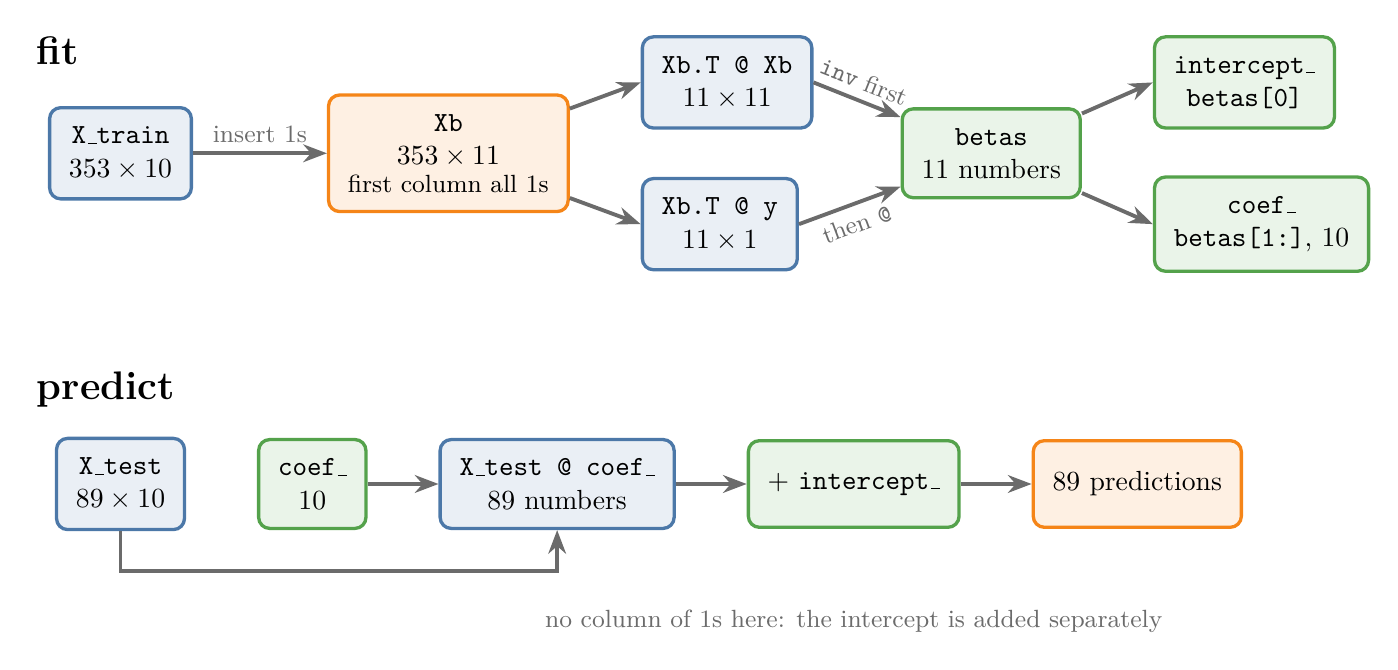
\begin{tikzpicture}[node distance=0.55cm and 0.9cm]
  \node[title, anchor=west] at (-1.2, 1.3) {fit};
  \node[box=cblue] (X) {\texttt{X\_train}\\$353 \times 10$};
  \node[box=corange, right=1.7cm of X] (Xb) {\texttt{Xb}\\$353 \times 11$\\[-2pt]{\small first column all 1s}};
  \node[box=cblue, right=of Xb, yshift=0.9cm] (XtX) {\texttt{Xb.T @ Xb}\\$11 \times 11$};
  \node[box=cblue, right=of Xb, yshift=-0.9cm] (Xty) {\texttt{Xb.T @ y}\\$11 \times 1$};
  \node[box=cgreen, right=1.2cm of Xb, xshift=3.0cm] (beta) {\texttt{betas}\\$11$ numbers};
  \node[box=cgreen, right=of beta, yshift=0.9cm] (b0) {\texttt{intercept\_}\\\texttt{betas[0]}};
  \node[box=cgreen, right=of beta, yshift=-0.9cm] (coef) {\texttt{coef\_}\\\texttt{betas[1:]}, $10$};
  \draw[arrow] (X) -- node[note, above] {insert 1s} (Xb);
  \draw[arrow] (Xb) -- (XtX.west);
  \draw[arrow] (Xb) -- (Xty.west);
  \draw[arrow] (XtX.east) -- node[note, above, sloped] {\texttt{inv} first} (beta);
  \draw[arrow] (Xty.east) -- node[note, below, sloped] {then \texttt{@}} (beta);
  \draw[arrow] (beta) -- (b0.west);
  \draw[arrow] (beta) -- (coef.west);
  % predict
  \node[title, anchor=west] at (-1.2, -3.0) {predict};
  \node[box=cblue] (Xt) at (0, -4.2) {\texttt{X\_test}\\$89 \times 10$};
  \node[box=cgreen, right=of Xt] (c2) {\texttt{coef\_}\\$10$};
  \node[box=cblue, right=of c2] (prod) {\texttt{X\_test @ coef\_}\\$89$ numbers};
  \node[box=cgreen, right=of prod] (i2) {$+$ \texttt{intercept\_}};
  \node[box=corange, right=of i2] (yh) {89 predictions};
  
  \draw[arrow] (c2) -- (prod);
  \draw[arrow] (Xt.south) -- ++(0,-0.5) -| (prod.south);
  \draw[arrow] (prod) -- (i2);
  \draw[arrow] (i2) -- (yh);
  \node[note, below=0.9cm of i2] {no column of 1s here: the intercept is added separately};
\end{tikzpicture}
\end{document}
